
% this file is called up by thesis.tex



\chapter{Material \& Metoder} % top level followed by section, subsection
\label{ch:metoder}

% ----------------------- paths to graphics ------------------------

% change according to folder and file names
\ifpdf
    \graphicspath{{8/figures/PNG/}{8_materials_and_methods/figures/PDF/}{8_materials_and_methods/figures/}}
\else
    \graphicspath{{8/figures/EPS/}{8_materials_and_methods/figures/}}
\fi

% ----------------------- contents from here ------------------------

\section{Material}
I vår lösning använde vi oss av ett utvecklingskort ESP8266 med ett inbyggt Wifi som var nödvändig för att kunna kommunicera med det nätverk som kameran var uppkopplad till.

Kameran är av modellen Q6128-E Network Camera med möjlighet till internetuppkoppling. Upplösningen som används är 3840x2860. Ett suffix med datum och tidsinformation läggs till i filnamnet för inspelningen.

En PIR-sensor från Adafruit användes som rörelsedetektor för att tända lampan i hållplatsen.

Som nämt tidigare i rapporten använde vi oss av en ljudsensor som var monterad mot en glasyta. Vid besök hos en elektrokit-grossist kunde vi inte få tag på någon användbar trycksensor som var tillräckligt känslig för att ersätta ljudsensorn. Under demo-dagen fick vi frågan om vi hade tänkt på en Piezo-sensor, som är en typ av en tryck-sensor. Efter fakta-sökning fann vi att en Piezo-sensor hade varit ett bättre alternativ än ljudsensorn.

För att kunna identifiera att någon har utfört vandalisering måste systemet lagra bilder/inspelningar på en server. En FTP-server användes. FTP-servern och IP-kameran låg i samma subnät.\\

Information om FTP-servern:

\begin{itemize}
\item IP adress : 192.168.0.106

\item Port nummer : 21

\item Användarnamn : ”FTP-User”

\item Lösenord : ”Safe24”

\end{itemize}

\begin{figure}[h]

  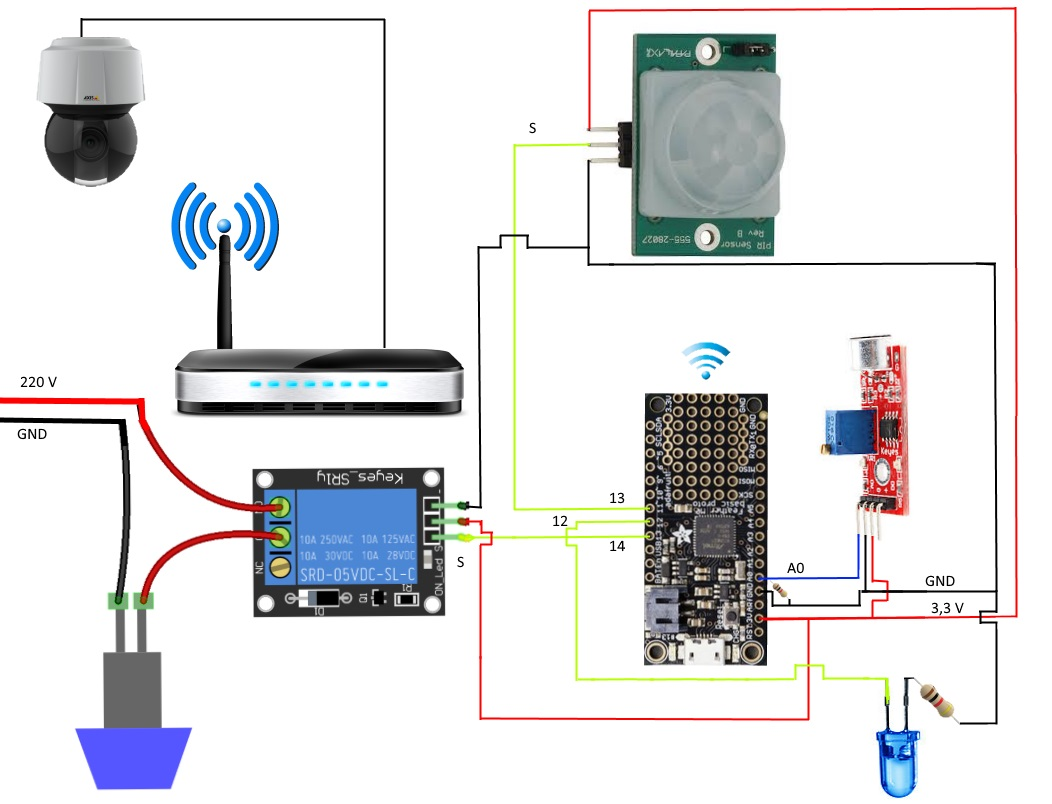
\includegraphics[width=\linewidth]{connections.jpg}
  \caption{Alla komponenter kopplade med varandra.)}
  \label{fig:connections}
\end{figure}
\clearpage



\section{Metoder} 
Om PIR-sensorn detekterar någon rörelse då skall lampan tändas en viss tid och sedan släckas. Om lampan är tänd och PIR-sensorn detekterar ny rörelse då fortsätter lampan vara tänd. För att lyckas med PIR-sensorn fick vi med hjälp av några delays och räknare räkna in hur många gånger som signalen var hög eller låg. Efter flera tester och försök kom vi fram till att det behövdes minst sju rundor med en runda på 0,5 sekunder. Anledningen till detta var att när det inte fanns någon rörelse så gav PIR-sensorn utslag med några ettor samt några nollor. Då det fanns rörelse gav den utslag på bara ettor.\\

 Ljud-sensorn är också igång hela tiden. Om ljudsensorn detekterar ett ljud som är över gränsvärdet skall den viktiga processen börja. På grund av brist på glas och utrymme för oss att göra testförsök med att ta sönder glas använde vi istället plast. Plasten skulle föreställa glaset i en busshållplats. Vi kom överens om att sätta tröskelvärdet till 75 utav max 1024 som analoga ingången kunde läsa. Över denna gräns indikerades att glas hade gått sönder.\\

IP-kameran var installerad i mitten av vägen så att den kan rotera fritt eftersom vandaliseringen kan ske på avstånd från hållplatsen. Den var ansluten via ethernet och vi styrde den med hjälp av http-kommando som utvecklingskortet skickade iväg. Vi fick kamerans http-API (VAPIX) från Axis. Inne i kameran skapade vi tre events ActionPTZStation1, ActionRecord, ActionPTZHome.

ActionPTZStation1: När virtuell port 8 aktiveras så riktas kameran mot en bestämd position som  heter "plats1" (busshållplatsen).

ActionRecord: När virtuell port 9 aktiveras så börjar kameran videoinspelningen. Efter avslutad inspelning skickas klippet till FTP-servern.

ActionPTZHome: När virtuell port 10 aktiveras så riktas kameran mot en bestämd position som heter Safe24 och som motsvarar start och slutpositionen för kameran.


 








\clearpage
\section{Systembeskrivning}
Vi har nämt tidigare i rapporten att vårt kamerasystem skall befinna sig i ett passivt läge så länge inget villkor är uppfyllt. Om ett villkor är uppfyllt då aktiveras två virtuella portar i kameran. Den ena riktar kameran mot busshållplatsen (port 8) och den andra (port 9) gör att kameran börjar filma. Då filmar kameran i fem sekunder och sedan filmar den runt omkring medan den vrider sig horisontellt. Efter ett varv riktas kameran mot busshållplatsen igen och det görs genom att aktivera virtuell port 9. Kameran ska forsätta filma några sekunder till och efter det ska den riktas mot sitt standardläge dvs ActionPTZHome. Den totala videolängden är 40 sekunder och filmen skickas till FTP-servern. Ifall ljudsensor detekterar ett annat ljud som är över gränsen inom 40 sekunder då ska processen börja från början dvs kameran riktas tillbaka mot bushållplatsen osv.\\
 Samtidigt som utvecklingskortet väntar på utslag från ljudsensorn, väntar den på utslag från PIR-sensorn. När någon rör sig inne i hållplatsen ser utvecklingskortet till att en lampa tänds och släcks en viss tidsperiod som hela tiden förlängs vid nya rörelser. I det fall där kamerasystemet aktiveras, tar kamerasystemet över PIR-sensorn och låter lampan att blinka tills kamerasystemet är tillbaka till sitt passiva läge.

\section{Arbetsuppgifter}
Gruppen arbetade både tillsammans och även enskilt så att var och en av gruppmedlemmarna kunde bidra med något. Benjamin var delaktig i arbetet med flödesdiagram, tasks, hjälp med byggandet av busshållplats och även testfall. Yurdaer arbetade med wifi-kodning av ESP:n, kamera-kommandon, ftp-servern och i rapporten skrev han om sina delar samt om etiska aspekter. Georges bidrag var med struktur av kod, API, manual, testfall, FTP-servern och en del rapportskrivning. Han bidrog även med upprättande av en Latex-mall för rapporten. Louay arbetade med sensorernas kodning, ihopkoppling av alla komponenter, förslag till router-lösning, byggandet av en hållplats och kontinuerlig testning av alla kopplingar. 
% ---------------------------------------------------------------------------
%: ----------------------- end of thesis sub-document ------------------------
% ---------------------------------------------------------------------------



 



